\chapter{State of the Art}
\label{chap:state_of_the_art}

This chapter presents a Systematic Literature Review (SLR) of the current landscape of Multi-Agent Systems (MAS) in software engineering. It details the methodology used for selecting studies, synthesizes findings regarding agent architectures and knowledge integration, and discusses the ethical implications of deploying autonomous agents in development workflows.


\section{Methodology}
\label{sec:methodology}


The rapid advancement of Large Language Models (LLMs) has precipitated a paradigm shift in Software Engineering (SE), particularly in the domain of automated software testing. While traditional automated testing relies heavily on static analysis and manually scripted test cases, the emergence of Generative AI (GenAI) offers the potential for autonomous, context-aware test generation. However, single-prompt LLM interactions often fail to address the complexity of enterprise-grade software due to hallucinations, limited context windows, and a lack of grounding in the execution environment. Consequently, the research frontier has moved towards Multi-Agent Systems (MAS), where specialized agents collaborate to plan, generate, execute, and refine tests.

This chapter presents a Systematic Literature Review (SLR) conducted to rigorously analyze the current state of the art in MAS-driven automated testing. Following the PRISMA 2020 guidelines \parencite{page2021prisma}, this review systematically identifies, selects, and synthesizes 25 primary studies published between 2023 and 2025. The goal is to answer critical questions regarding the architectural orchestration of these agents, the integration of domain-specific knowledge, and the validation methodologies used to ensure reliability. Furthermore, this chapter includes a dedicated analysis of the ethical, legal, and environmental implications of deploying autonomous agents in software development workflows.

To ensure transparency, reproducibility, and scientific rigor, this SLR adopts a structured methodology based on the PRISMA (Preferred Reporting Items for Systematic Reviews and Meta-Analyses) framework. The review process was executed in four distinct phases: (1) Definition of Research Questions, (2) Search Strategy, (3) Study Selection, and (4) Data Extraction and Synthesis.

\section{Research Questions}
The primary objective of this review is to understand how MAS architectures can overcome the limitations of monolithic LLMs in software testing. To this end, three specific Research Questions (RQs) were formulated, as detailed in Table \ref{tab:research_questions}.

\begin{table}[h]
\caption{Research Questions}
\label{tab:research_questions}
\centering
\begin{tabular}{l p{10cm}}
\toprule
ID & Research Question \\
\midrule
RQ1 & Architecture \& Orchestration: How are specialized agents within Multi-Agent Systems architecturally decomposed, coordinated, and orchestrated to accomplish complex software testing tasks? \\
\midrule
RQ2 & Knowledge Integration: What methodologies (e.g., Retrieval-Augmented Generation, Tool Use, Agent-Computer Interfaces) are employed to integrate proprietary, domain-specific knowledge into LLM-based test generation systems? \\
\midrule
RQ3 & Validation \& Evaluation: How do existing studies evaluate the correctness, coverage, and effectiveness of LLM-generated test scripts, and what benchmarks are considered the gold standard? \\
\bottomrule
\end{tabular}
\end{table}

\section{Search Strategy}
\label{sec:search_strategy}

\subsubsection{Data Sources}
Given the rapid pace of development in Generative AI, the search was conducted across the following major academic databases (see Table \ref{tab:datasources}).

\begin{table}[h]
\caption{Selected Data Sources}
\label{tab:datasources}
\centering
\begin{tabular}{l p{10cm}}
\toprule
Database & Justification \\
\midrule
Semantic Scholar & To identify citation networks and relevant peer-reviewed papers in venues such as ICSE, FSE, and ASE. \\
\midrule
IEEE Xplore & To ensure coverage of formally published archival literature in engineering and computer science. \\
\midrule
ACM Digital Library & To capture high-impact proceedings from major computing conferences. \\
\bottomrule
\end{tabular}
\end{table}

\subsubsection{Search Strings}
To ensure a comprehensive retrieval of relevant studies, a multi-string search strategy was employed. Instead of a single broad query, three distinct boolean search strings were constructed to target specific dimensions of the research questions, as detailed in Table \ref{tab:search_strings}.

\begin{table}[h]
\caption{Search Strings Strategy}
\label{tab:search_strings}
\centering
\begin{tabular}{l p{3cm} p{9cm}}
\toprule
ID & Scope & Search String \\
\midrule
S1 & Core Scope & ("Software Testing" OR "Test Generation" OR "Unit Testing" OR "Fuzzing" OR "Regression Testing" OR "Test Maintenance") AND ("Multi-Agent" OR "MAS" OR "Agentic" OR "Autonomous Agents") AND ("LLM" OR "Large Language Model" OR "Generative AI" OR "GenAI") \\
\midrule
S2 & Validation & ("Software Testing") AND ("LLM" OR "Agent") AND ("Benchmark" OR "SWE-bench" OR "HumanEval" OR "Pass@k" OR "Code Coverage" OR "Self-Correction") \\
\midrule
S3 & Ethics \& Cost & ("Software Engineering") AND ("LLM" OR "Agent") AND ("Privacy" OR "GDPR" OR "Data Leakage" OR "Bias" OR "Energy Consumption" OR "Green AI") \\
\bottomrule
\end{tabular}
\end{table}

The search was conducted in December 2025, covering the period from January 2023 to December 2025. This timeframe was selected to focus specifically on the "post-ChatGPT" era, where agentic capabilities became viable.

\section{Inclusion and Exclusion Criteria}
The selection process was governed by rigorous inclusion and exclusion criteria to ensure the relevance and quality of the selected studies, as defined in Table \ref{tab:inclusion_criteria}.

\begin{table}[h]
\caption{Inclusion and Exclusion Criteria}
\label{tab:inclusion_criteria}
\centering
\begin{tabular}{l p{10cm}}
\toprule
ID & Criterion \\
\midrule
IC1 & Population: Software development environments, focusing on code repositories and testing workflows. \\
IC2 & Intervention: Multi-Agent Systems (MAS) utilizing LLMs as the reasoning engine. \\
IC3 & Outcome: Quantitative metrics such as Pass@k, Code Coverage, or Qualitative assessments. \\
\midrule
EC1 & Papers focused solely on single-prompt engineering without agentic loops. \\
EC2 & Studies lacking empirical validation or reproducible benchmarks. \\
EC3 & Non-English publications. \\
EC4 & Grey literature not backed by technical reports. \\
\bottomrule
\end{tabular}
\end{table}

\section{Study Selection Process}
The systematic search process yielded a total of 239 records across the selected databases. After removing duplicates (9), 230 unique citations were screened based on title and abstract. This initial screening led to the exclusion of 190 records that did not meet the population or intervention criteria (e.g., general NLP papers, non-SE applications). The remaining 40 full-text articles were assessed for eligibility. Of these, 18 were excluded for reasons such as lack of empirical validation (EC2) or focus on single-agent prompting (EC1). The final set comprises 22 primary studies that form the basis of the synthesis presented in Section \ref{sec:results}. The selection flow is illustrated in Figure \ref{fig:prisma_flow}.

% Auto-generated table rows
MAGISTER: LLM-Based Test Generation with Role-Specialized Agents & 2025 International Conference on Intelligent Systems: Theories and Applications (SITA) & 2025 \\ \hline
A Vision for Debiasing Confirmation Bias in Software Testing via LLM & 2025 ACM/IEEE International Symposium on Empirical Software Engineering and Measurement (ESEM) & 2025 \\ \hline
Evaluation of the Choice of LLM in a Multi-Agent Solution for GUI-Test Generation & 2025 IEEE Conference on Software Testing, Verification and Validation (ICST) & 2025 \\ \hline
MultiFuzz: A Dense Retrieval-based Multi-Agent System for Network Protocol Fuzzing & 2025 IEEE/ACS 22nd International Conference on Computer Systems and Applications (AICCSA) & 2025 \\ \hline
MCM: A Multi-Agent Collaborative Multimodal Framework For Traditional Chinese Medicine Diagnosis & 2025 IEEE International Conference on Image Processing (ICIP) & 2025 \\ \hline
HPCAgentTester: a Multi-Agent LLM Approach for Enhanced HPC Unit Test Generation & 2025 2nd IEEE/ACM International Conference on AI-powered Software (AIware) & 2025 \\ \hline
LibLMFuzz: LLM-Augmented Fuzz Target Generation for Black-Box Libraries & 2025 Cyber Awareness and Research Symposium (CARS) & 2025 \\ \hline
LLM-Driven Smart Test Case Generation for Scalable Software Testing & 2025 2nd International Conference on Software, Systems and Information Technology (SSITCON) & 2025 \\ \hline
AI-Powered Multi-Agent Framework for Automated Unit Test Case Generation: Enhancing Software Quality through LLM’s & 2024 5th IEEE Global Conference for Advancement in Technology (GCAT) & 2024 \\ \hline
IntelliTest: An Intelligent Framework for Agentic Functional Test Generation Using Multimodal Data and Domain Knowledge & 2025 IEEE Future Networks World Forum (FNWF) & 2025 \\ \hline
Multi-Agent Auditing for Smart Contracts* & 2025 9th International Symposium on Computer Science and Intelligent Control (ISCSIC) & 2025 \\ \hline
An Agentic Reasoning-Based Feedback System for Programming Assignments & 2025 IEEE 11th International Conference on Computing, Engineering and Design (ICCED) & 2025 \\ \hline
LLMs in Debate: Does Arguing Make Them Better at Detecting Metamorphic Relations? & 2025 40th IEEE/ACM International Conference on Automated Software Engineering Workshops (ASEW) & 2025 \\ \hline
Human-In-The-Loop Software Development Agents: Challenges and Future Directions & 2025 IEEE/ACM 22nd International Conference on Mining Software Repositories (MSR) & 2025 \\ \hline
Seeing is Believing: Vision-Driven Non-Crash Functional Bug Detection for Mobile Apps & IEEE Transactions on Software Engineering & 2025 \\ \hline
Research on Multi-Model Fusion Machine Learning Demand Intelligent Forecasting System in Cloud Computing Environment & 2025 2nd International Conference on Intelligent Algorithms for Computational Intelligence Systems (IACIS) & 2025 \\ \hline
Unit Test Generation Multi-Agent AI System for Enhancing Software Documentation and Code Coverage & 2024 32nd Telecommunications Forum (TELFOR) & 2024 \\ \hline
Large Language Model Supply Chain: A Research Agenda & TOSEM '25 & 2025 \\ \hline
A Survey on Large Language Models for Code Generation & TOSEM & 2026 \\ \hline
RepairAgent: An Autonomous, LLM-Based Agent for Program Repair & ICSE '25 & 2025 \\ \hline
Demystifying LLM-Based Software Engineering Agents & PACMSE (FSE) & 2025 \\ \hline
A Multi-Agent Approach for REST API Testing with Semantic Graphs and LLM-Driven Inputs & ICSE '25 & 2025 \\ \hline


\begin{figure}[h]
    \centering
    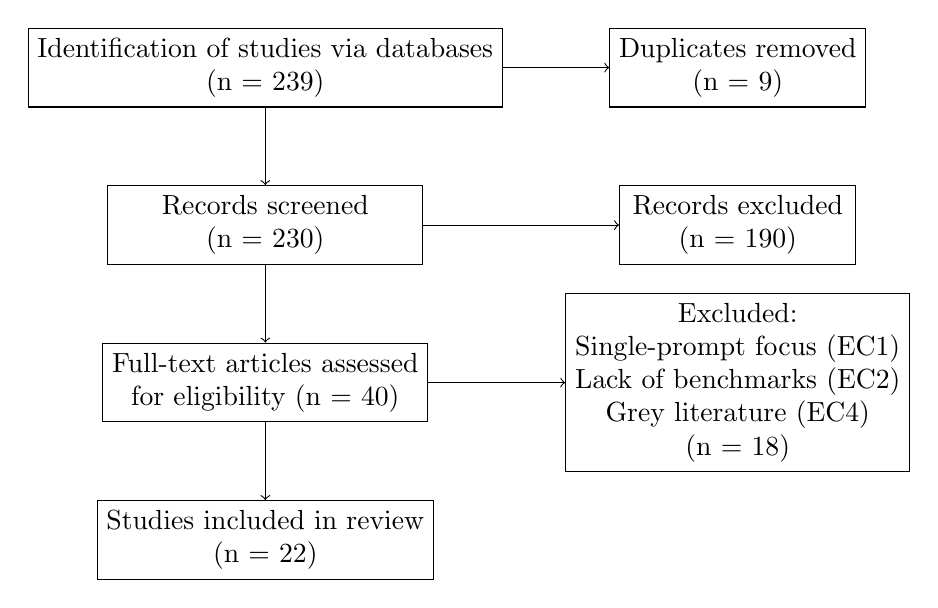
\begin{tikzpicture}[node distance=2cm]
        \node (identification) [draw, rectangle, minimum width=4cm, minimum height=1cm, align=center] {Identification of studies via databases\\(n = 239)};
        \node (screening) [draw, rectangle, below of=identification, minimum width=4cm, minimum height=1cm, align=center] {Records screened\\(n = 230)};
        \node (duplicates) [draw, rectangle, right of=identification, xshift=4cm, minimum width=3cm, minimum height=1cm, align=center] {Duplicates removed\\(n = 9)};
        \node (excluded_screen) [draw, rectangle, right of=screening, xshift=4cm, minimum width=3cm, minimum height=1cm, align=center] {Records excluded\\(n = 190)};
        \node (eligibility) [draw, rectangle, below of=screening, minimum width=4cm, minimum height=1cm, align=center] {Full-text articles assessed\\for eligibility (n = 40)};
        \node (excluded_full) [draw, rectangle, right of=eligibility, xshift=4cm, minimum width=3cm, minimum height=1cm, align=center] {Excluded:\\Single-prompt focus (EC1)\\Lack of benchmarks (EC2)\\Grey literature (EC4)\\(n = 18)};
        \node (included) [draw, rectangle, below of=eligibility, minimum width=4cm, minimum height=1cm, align=center] {Studies included in review\\(n = 22)};

        \draw[->] (identification) -- (screening);
        \draw[->] (identification) -- (duplicates);
        \draw[->] (screening) -- (eligibility);
        \draw[->] (screening) -- (excluded_screen);
        \draw[->] (eligibility) -- (included);
        \draw[->] (eligibility) -- (excluded_full);
    \end{tikzpicture}
    \caption{PRISMA 2020 Flow Diagram for the Systematic Literature Review.}
    \label{fig:prisma_flow}
\end{figure}


\section{Quality Assessment}
Each selected study was evaluated for quality based on three factors: (1) Reproducibility (availability of code/datasets), (2) Benchmarking (use of standard benchmarks like SWE-bench vs. ad-hoc datasets), and (3) Architectural Clarity (clear definition of agent roles and communication protocols).

\section{Synthesis of Findings}
\label{sec:results}

This section synthesizes the findings from the selected primary studies, structured according to the three research questions defined in the methodology. It begins by analyzing the architectural patterns of MAS, explores the mechanisms for integrating domain knowledge, and concludes with an assessment of validation strategies.

\subsection{RQ1: Architecture \& Orchestration}
The literature reveals a decisive move from single-agent systems to multi-agent architectures. The synthesis identifies two primary architectural patterns: Hierarchical and Cooperative orchestration.

\subsubsection{Hierarchical Orchestration (Waterfall)}
In hierarchical systems, agents are organized in a top-down structure mimicking a corporate hierarchy. \textcite{ahammad2025magister} introduced MAGISTER, a role-based framework where specialized agents (Analyzer, Generator, Executor, Refiner) collaborate in a linear workflow. The Analyzer identifies testable units, passing structured specifications to the Generator, whose output is validated by the Executor. This linear hand-off ensures that each agent operates within a narrow, well-defined context, reducing hallucinations. Similarly, \textcite{ding2025multiagent} proposed Multi-Agent Auditing (MAA) for smart contracts, employing a constrained protocol where a "Manager" agent orchestrates "Auditor" agents, privileging verifiable artifacts over free-form dialogue.

\subsubsection{Cooperative Orchestration (Feedback Loops)}
Cooperative architectures focus on iterative refinement through peer review and debate. \textcite{tomic2025evaluation} explored this with PathFinder, a framework for GUI testing where agents (Perception, Decision, Action) work collaboratively. Their study evaluated significantly different LLM combinations (e.g., Llama vs. Mistral) for different roles, finding that heterogeneous agent teams often outperform homogenous ones. \textcite{bose2025llms} demonstrated that a "Multi-Agent Debate" mechanism, where agents argue about the validity of a test case (specifically metamorphic relations), significantly improves the stability and correctness of test generation compared to single-model reasoning.

\subsubsection{Self-Reflection and Debugging}
Recent works emphasize "Self-Reflection" loops. \textcite{karanjai2025hpcagenttester} introduced HPCAgentTester for High-Performance Computing (HPC), which uses a "Critique Loop" where a Test Agent and a Recipe Agent iteratively refine MPI/OpenMP test cases until compilation succeeds. This iterative refinement is crucial for domains where syntax is strict. Similarly, \textcite{salman2025a} addressed cognitive biases in testing, proposing a vision where agents utilize "Debiasing" strategies to reduce confirmation bias in test case design. \textcite{kanagaraj2025llmdriven} and \textcite{garlapati2024aipowered} further validated this by employing Chain-of-Thought (CoT) reasoning to produce context-aware test suites that achieve over 85\% code coverage. \textcite{stojanović2024unit} extended this to Behavior-Driven Development (BDD), using a three-agent system to generate user stories and corresponding unit tests, thereby linking requirements directly to implementation.

\subsection{RQ2: Knowledge Integration}
A critical limitation of off-the-shelf LLMs is their lack of knowledge about specific enterprise codebases. The review identifies two dominant strategies for knowledge integration: Retrieval-Augmented Generation (RAG) and Agent-Computer Interfaces (ACI).

\subsubsection{Retrieval-Augmented Generation (RAG)}
RAG allows agents to query external knowledge bases. \textcite{maklad2025multifuzz} introduced MultiFuzz, a dense retrieval-based system for network protocol fuzzing. By retrieving relevant RFC chunks and protocol grammars, MultiFuzz enables agents to generate valid inputs for complex state machines (e.g., RTSP), significantly outperforming traditional fuzzers like AFLNet. Similarly, \textcite{tiwari2025intellitest} proposed IntelliTest, which uses an ontology-driven RAG approach. It constructs a "specification knowledge graph" from software change artifacts, allowing agents to retrieve semantic dependencies rather than just keyword matches. This structured retrieval is essential for large-scale embedded systems.

\subsubsection{Agent-Computer Interfaces (ACI)}
The concept of ACI provides agents with executable tools. \textcite{hardgrove2025liblmfuzz} demonstrated LibLMFuzz, where an agent drives a toolchain to fuzz black-box libraries. \textcite{pasuksmit2025humanintheloop} emphasized the importance of tool feedback in resolving Jira tickets. This tool-use paradigm is also evident in program repair. \textcite{bouzenia2025repair} introduced RepairAgent, which uses a finite state machine to plan and execute actions/tools to fix bugs autonomously. In the API testing domain, \textcite{kim2024multi} proposed a multi-agent approach for REST API testing that uses semantic graphs and reinforcement learning to generate valid inputs, effectively acting as an ACI for the web layer.

\subsection{RQ3: Validation \& Evaluation}
Validating the output of generative models is notoriously difficult. The SLR highlights a transition from static similarity metrics (e.g., BLEU score) to execution-based functional correctness and "stability" metrics.

\subsubsection{Benchmarks: From HumanEval to Real-World}
While early studies relied on toy datasets, recent work focuses on real-world complexity. \textcite{pasuksmit2025humanintheloop} highlight that agents must be evaluated on their ability to resolve actual issue tickets (e.g., Jira), not just synthetic prompts. They propose using functional correctness testing (Pass@1) on real repositories as the gold standard. \textcite{kanagaraj2025llmdriven} validated their framework on diverse applications, achieving 85.3\% code coverage, demonstrating that coverage remains a primary metric for industrial adoption.

\subsubsection{Stability as a Metric}
Beyond correctness, "stability" is emerging as a critical metric. \textcite{bose2025llms} argue that LLMs should be evaluated on their consistency in identifying metamorphic relations. Their "debate" mechanism improved this stability. \textcite{sulaiman2025an} introduced "Explain-then-Grade", showing that requiring agents to explain their reasoning improves alignment with human judgements. \textcite{xia2024agentless} challenged the complexity of agents in "Demystifying LLM-Based Software Engineering Agents", showing that simpler, "Agentless" approaches can sometimes outperform complex agentic frameworks if the prompt engineering is robust. This highlights a tension in the field between architectural complexity and raw model capability.

\subsubsection{Domain-Specific Validation}
Validation strategies must be tailored to the domain. \textcite{liu2025seeing} proposed VisionDroid for mobile GUI testing, using Multimodal LLMs to detect non-crash functional bugs essentially by "looking" at the screenshots, a capability absent in traditional tools. \textcite{huang2025research} discussed evaluating LLMs in cloud demand forecasting contexts, noting that while LLMs improve unit test generation, their performance varies significantly across different datasets and tasks. Finally, broad surveys by \textcite{jiang2024survey} and \textcite{wang2025supply} underscore that the "LLM Supply Chain"—from foundation model training to downstream agent deployment—introduces variability that must be accounted for in any rigorous evaluation.

\section{Discussion}
\label{sec:discussion}

The analysis of the state of the art reveals a clear trajectory in automated software testing: the move from static, brittle scripts to dynamic, agentic workflows. However, this transition is not without its challenges. The primary problem identified in the literature is the reliability of agentic code generation in large-scale environments. While agents like those in \cite{ahammad2025magister} perform well on modular Python projects, they struggle with "Contextual Blindness" when modifying existing brownfield repositories \cite{tiwari2025intellitest}.

This dissertation aims to solve this specific problem by implementing an enhanced ACI that provides agents with "spatial awareness" of the codebase—allowing them to map dependencies before attempting modifications. Unlike existing approaches that rely on naive RAG \cite{maklad2025multifuzz}, our proposed solution will integrate a semantic code graph to guide the agent's navigation. Furthermore, the "Search-based" strategies discussed in \cite{hardgrove2025liblmfuzz} will be adapted to ensure that the system can autonomously recover from the compilation errors that currently plague single-shot generations. By closing the loop between generation and execution, we expect to achieve a significant improvement in the Pass@1 metric for real-world issues.

\section{Conclusion}
\label{sec:conclusion_sota}

This Systematic Literature Review confirms that the integration of Multi-Agent Systems with Large Language Models represents a transformative leap in automated software testing. By decomposing tasks, integrating external tools via ACIs, and employing rigorous execution-based validation, MAS architectures address the key limitations of hallucinations and lack of context that plagued earlier single-agent approaches. However, significant challenges regarding data privacy, legacy language support, and energy efficiency must be addressed before widespread enterprise adoption is feasible. The findings of this review directly inform the design of the framework proposed in this dissertation.
